\documentclass[12pt,fleqn]{article}
\usepackage{a4}
\usepackage{graphicx}
\graphicspath{ {./Figures/} }
\usepackage{psfrag}
\usepackage{amsmath}                     % \boldsymbol{#1}
\usepackage{amssymb}
\usepackage{Styles/hangcaption}
\usepackage{Styles/pstricks}
\usepackage{Styles/pst-node}
\usepackage{Styles/fancyheadings}
\usepackage{tocloft}
\usepackage{cite}
\usepackage{hyperref}
\usepackage[printonlyused]{acronym}
\usepackage{epstopdf}
\usepackage{advdate}
\hypersetup{
    colorlinks=false,
    linkcolor=black,
    filecolor=black,      
    urlcolor=black,
    }
    
\newcommand{\yesthreeday}{{\AdvanceDate[-4]\today}}
\epstopdfDeclareGraphicsRule{.pdf}{png}{.png}{convert #1\OutputFile}
\DeclareGraphicsExtensions{.png,.pdf}

%-----Tex width---------------------------------
\textwidth 16cm

%-----Line spacing-------------------------------
\renewcommand{\baselinestretch}{1.5}     % 1,1-zeilig

%---------Add dots in TOC-----------------------
\renewcommand{\cftsecleader}{\cftdotfill{\cftdotsep}}

%------Paragraph indention-------------------------------
\setlength{\parskip}{1.5ex plus0.5ex minus0.5ex}

%-----Prevent indent----------------------
\setlength{\parindent}{0em}

%-----Richtiger Abstand fur Einheiten-------------
\def\Unit{\hspace{0.25em}}

%-----Definition of the header--------------------
\pagestyle{fancyplain}
\renewcommand{\sectionmark}[1]{\markboth{Chapter~\thesection.~#1}{#1}}
\renewcommand{\subsectionmark}[1]{\markright{\thesubsection\ #1}}
\rhead[\fancyplain{}{\leftmark}]%
{\fancyplain{\thepage}{\thepage}} \cfoot{} \plainheadrulewidth
0.4pt
%% Otherwise: Overfull \vbox-Warning against fancyheadings-pacakage
%%  idea of: nic@minster.york.ac.uk (Nick Cropper)
\makeatletter
\ifcase \@ptsize \relax % 10pt
  \addtolength{\headheight}{1\p@}
\or % 11pt
  \addtolength{\headheight}{2\p@}
\or % 12pt
  \addtolength{\headheight}{3\p@}
\fi \makeatother

%-----Equations / Figures / Tables numbering according to \ sections
\makeatletter
\renewcommand\theequation{\thesection.\arabic{equation}}
\renewcommand\thefigure{\thesection.\arabic{figure}}
\renewcommand\thetable{\thesection.\arabic{table}}
\@addtoreset{equation}{section} \@addtoreset{figure}{section}
\@addtoreset{table}{section} \makeatother

%-----Useful abbreviations----------------------
\newcommand{\mr}{\mathrm}
\newcommand{\bs}[1]{\mbox{$\boldsymbol{#1}$}}
\newcommand{\degree}[1]{\mbox{$#1^\circ$}}

%\renewcommand{\figurename}{Bild}

%------Bibliography style-----------------------
\bibliographystyle{IEEEtran}

%-----Aufzaehlunstiefe im Literaturverzeichnis---------------
\setcounter{tocdepth}{3}

\begin{document}
\pagenumbering{Roman}
\begin{titlepage}
  \begin{center}
      \vspace*{-4.0cm}
    \begin{figure}[!h]
\centering

\includegraphics[width=0.3\linewidth]{Figures/JKUAT_logo}
%\caption{}
\label{fig:jomologo}
\end{figure}
   \large{Jomo Kenyatta University of Agriculture and Technology}\\
    \large{College of Engineering and Technology}\\
    \large{School of Mechanical, Materials, and Manufacturing Engineering}\\
   \large{Department of Mechatronic Engineering}\\

    ------------------------------------------------------------------------------------------------\\[1.0cm]
    \LARGE{\textbf{Design and Fabrication of an Internet of Things Level-4 Autonomous Smart Fan}}\\[0.6cm]
    
    \LARGE{\textbf{Final year project proposal
            }}\\[1.5cm]
    %\large{by}\\[0.6cm

    \vspace{0.5cm}
    \large{\textbf{Gitu Kelvin Karimi (ENM221-0058/2017)
            }}\\
     \large{\textbf{Osodo Rodney David (ENM221-0091/2017)
            }}\\[1.0cm]

    % \large{\small{\today}}\\
    \large{\small{\yesthreeday}}\\
    ------------------------------------------------------------------------------------------------\\[1.5cm]
  \end{center}
\end{titlepage}
%
%\pagenumbering{gobble}% Remove page numbers (and reset to 1)

\addcontentsline{toc}{section}{Declaration}
\section*{Declaration}


We hereby declare that the work contained in this report is original; researched and documented by the undersigned students. It has not been used or presented elsewhere in any form for award of any academic qualification or otherwise. Any material obtained from other parties have been duly acknowledged. We have ensured that no violation of copyright or intellectual property rights have been committed.
\begin{enumerate}
	\item Gitu Kelvin Karimi\vspace*{.2cm}\\
	Signature\ldots\ldots\ldots\ldots\ldots\ldots\ldots\ldots\ldots\ldots Date\ldots\ldots\ldots\ldots\ldots\ldots\ldots\ldots\ldots\ldots
	\item Osodo Rodney David\vspace*{.2cm}\\
	Signature\ldots\ldots\ldots\ldots\ldots\ldots\ldots\ldots\ldots\ldots Date\ldots\ldots\ldots\ldots\ldots\ldots\ldots\ldots\ldots\ldots
\end{enumerate}

\vspace*{.5cm}
Approved by supervisor:
\begin{enumerate}
	\item Eng. Macben M. Mackenzie\vspace*{.2cm}\\
	Signature\ldots\ldots\ldots\ldots\ldots\ldots\ldots\ldots\ldots\ldots Date\ldots\ldots\ldots\ldots\ldots\ldots\ldots\ldots\ldots\ldots
\end{enumerate}



\clearpage
\tableofcontents
\clearpage
% \addcontentsline{toc}{section}{Table of Contents}
\addcontentsline{toc}{section}{List of Figures}
%{%
\let\oldnumberline\numberline%
\renewcommand{\numberline}{\figurename~\oldnumberline}%
\listoffigures
\clearpage
\addcontentsline{toc}{section}{List of Tables}
\listoftables
\newpage
\clearpage
\addcontentsline{toc}{section}{List of Abbreviations}
\linespread{1.0}
\setlength{\parskip}{0.1em}
\section*{List of Abbreviations}
% Some text \ac{USA}

\begin{acronym}
 \acro{DC} {Direct Current}
\end{acronym}
\begin{acronym}
 \acro{UN} {United Nations}
\end{acronym}
\begin{acronym}
 \acro{SDG} {Sustainable Development Goals}
\end{acronym}
\begin{acronym}
 \acro{DAC} {Digital to Analog Converter}
\end{acronym}
\begin{acronym}
 \acro{PWM} {Pulse Width Modulation}
\end{acronym}
\begin{acronym}
 \acro{SLAM} {Simultaneous Localization and Mapping}
\end{acronym}
\begin{acronym}
 \acro{LIDAR} {Light Detection and Ranging}
\end{acronym}

\clearpage
\newpage

\addcontentsline{toc}{section}{Abstract}

\section*{Abstract}
\label{sec:Abstract}

There is a rise in temperatures due to global warming and everyone is bestowed with the responsibility to reduce and possibly eradicate global warming. We too should take part in temperature regulations especially in Sub Saharan Africa so as to dampen the effect of global warming. Most common temperature regulation devices, air conditioners and fans are inefficient. Air conditioners use a lot of energy. On the other hand, most fans are manual and the smart ones are not smart enough to stop themselves in the absence of humans thereby using energy unsparingly.
\par
This project, therefore, proposes an \ac{IoT} level 4 autonomous fan system that would sense when the temperature is going up and sense the presence of people in the room and turn itself on. If the occupants leave it would automatically turn off. We intend to reduce the energy cost used in cooling houses thereby ensuring a sustainable energy consumption pattern while at large, building up sustainable cities.
\par
This system would have sensor nodes positioned at different endpoints in the room that measure the temperature of the room. The fan will only start if there are people in the room and if the temperature increases above a normal preset temperature, the fan will start running. It will adjust its speed of rotation based on the temperature difference. This will be detected by a sensor on the smart fan main unit. If people walk out the fan will sense this and stop. Generally, the fan is specified to operate between a predefined working schedule by the homeowner.
\par
This project intends to develop a smart fan product that will be applicable in society and apply for certification at the \ac{KEBS}.

\clearpage
\pagenumbering{arabic}
  \section{Introduction}
\subsection{Background}
(Insert your content)
\subsection{Problem statement}
(Insert your content)
\subsection{Objectives}
(Insert your content)
\subsection{Justification of the study}
(Insert your content)
  \clearpage
  \section{Literature Review}

\label{sec:review}

\subsection{Introduction}

The majority of mobile platforms or unmanned vehicles in use today are non-holonomic.
They only have one or two degrees of freedom that are independent.
As a result, its maneuverability is limited, and it frequently requires a large amount of space to control functions such as turning and parking.
This can be seen when a car wants to turn 180\degree.
By increasing a vehicle's degrees of freedom we are improving its maneuverability.
It can follow many complex trajectories that conventional nonholonomic vehicles find difficult or impossible.
Holonomic refers to the relationship between controllable and total degrees of freedom of a robot.
A holonomic platform is any mobile platform with three independent degrees of freedom in a plane.
If the controllable degree of freedom is equal to the total degrees of freedom, then the robot is said to be holonomic.
Independent degrees of freedom indicate that it can change its orientation or position without affecting other motions, as opposed to car-type vehicles, which must turn or change their orientation when moving.
A robot built on castor wheels or Omni-wheels is a good example of a holonomic drive as it can freely move in any direction and the controllable degrees of freedom is equal to total degrees of freedom. 


\subsubsection{Mobile platforms}

Over the last three decades, researchers have been working on omnidirectional wheeled mobile robots.
There are also legged mobile robots which achieve both holonomic and omnidirectional motion.
Legged mobile platforms have the advantage of highly adapted to uneven terrain, low soil interaction and the ability to perform tasks in congested and narrow environments.
Nevertheless, their slow mobility, low payload weigh to mechanism weight ratio, complex design and control makes them difficult to find\cite{seeni_2008}.

\subsubsection{Castor Wheel}

A castor or caster wheel is a relatively free-rolling ,not powered, small undriven wheel.
They are designed to be attached to the bottom of a larger object, to enable easy movement across a floor or other hard surface.
Castor wheels are manufactured in either a single wheel, double wheel, or compound wheel configuration.
\par
Most castors are used simply to make a heavy or cumbersome piece of furniture or machinery - the vehicle - easier to move.
Affixing small, unobtrusive wheels to the bottom of any large or bulky item is a great way to make it more mobile in certain scenarios.
In most cases, they are attached to the underside of the vehicle via a fixed top plate, from which the wheel assembly hangs.
\par
When choosing the type of casters to use in an application, weight considerations need to be considered depending on the load the casters will be required to move.
To achieve this, we need to consider the weight of the item being supported as shown by equation \ref{eq:1}.

\begin{equation}
\label{eq:1}
total\:load\:capacity = individual\:weight\:rating * number\:of\:wheels
\end{equation}

The total load-bearing capacity of your castors should always be at least 30\% higher than the total weight of the item when fully loaded, to give a sufficient safety margin.
Another consideration to take into account is the type of surface the castors will be moving on.
These surfaces are either flat and smooth that can accommodate small wheels or rougher surfaces that require wheels with larger diameters.
There are several types of castors each suited to a different application.
The most common casters are as shown by figure \ref{fig:polyurethanecastorwheels}, figure \ref{fig:synthetictreadwheels} and figure \ref{fig:ferrouscasterwheels}

\begin{figure}[htbp]
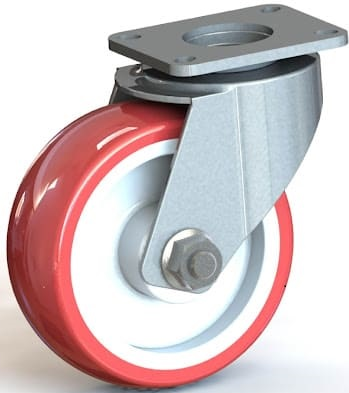
\includegraphics[scale=0.3]{Figures/polyurethane-caster-wheel.png}
\centering
\caption[Polyurethane Castor Wheels] {Polyurethane Castor Wheels	 \cite{noauthor_caster_nodate}.}
\label{fig:polyurethanecastorwheels}
\end{figure}

\begin{figure}[htbp]
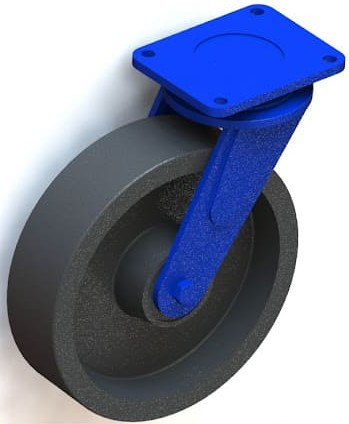
\includegraphics[scale=0.3]{Figures/synthetic-tread-wheels.jpg}
\centering
\caption[Synthetic Tread Wheels] {Synthetic Tread Wheels	 \cite{noauthor_caster_nodate}.}
\label{fig:synthetictreadwheels}
\end{figure}

\begin{figure}[htbp]
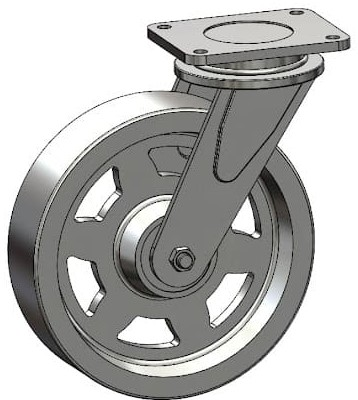
\includegraphics[scale=0.3]{Figures/ferrous-caster-wheel.jpg}
\centering
\caption[Ferrous Caster Wheels] {Ferrous Caster Wheels	 \cite{noauthor_caster_nodate}.}
\label{fig:ferrouscasterwheels}
\end{figure}

Ferrous wheels, Figure \ref{fig:ferrouscasterwheels} provide the highest load capacity, impact resistance, temperature range, and rollability of any caster wheel available due to their solid structure, making them excellent for harsh situations such as warehouses and manufacturing factories where a floor protection is not a priority.
Polyurethane tread wheels, Figure \ref{fig:polyurethanecastorwheels} provide good floor protection and have a 3,000-pound capacity and strong impact resistance \cite{noauthor_caster_nodate}.
Synthetic wheels Figure \ref{fig:synthetictreadwheels}, have a harder tread with lower rolling resistance and higher impact strength and reliability.
While most synthetic wheels are ideal for high-impact and harsh situations, they are louder than softer materials and are less forgiving when colliding with debris. 

\subsection{Existing Technologies}

\subsubsection{Wheel design}

For wheeled mobile robots, we have \cite{muir_kinematic_1987}: conventional wheels, omnidirectional wheels, and ball wheels.
The conventional wheels are the ones we see on cars and trolleys every day.
An omnidirectional wheel is a disk-shaped wheel with numerous conventional wheels mounted on its periphery.
A ball wheel \cite{ostrovskaya_dynamics_2000}, \cite{west_design_1995} is shaped like a ball but its implementation is difficult because including an axle in the design sacrifices usable workspace.
It is also difficult to provide power transmission to the wheel.
For large and heavy outdoor robots, four-wheel or car-like driving mechanisms have traditionally been used.
Because the non-holonomic constraints on their wheel mechanisms prevent sideways movements, these vehicles are quite restricted in their motion \cite{laumond_feasible_1986}\cite{pin_autonomous_1990}\cite{noauthor_navigation_nodate}, especially when operating in tight environments.
Improved motion capabilities have been investigated in a number of research centers and demonstrated on laboratory robots.
These motion capability enhancements are typically derived from the use of two independent driving wheels supplemented by casters.
This allows the platform to rotate around any point but does not allow for sideways motion.
Another motion can be achieved using two steerable and independently driving wheels \cite{pin_autonomous_1989}, or three steerable and coordinated driving wheels \cite{pin_autonomous_1989}.
These two implementations allow for both platform rotation and sideways motion through coordinated steering of the wheels.
However, in these latter systems, the controls for translational and rotational motions are not fully decoupled or independent, as very strict compatibility conditions exist between the steering and driving velocities of the wheels \cite{alexander_kinematics_1989}.
To achieve the full three degrees of freedom of planar rigid body motion, these platforms must be controlled as strongly constrained systems.
Furthermore, steering necessitates the rotation of the wheels around a vertical axis, which, in the case of heavy payloads or vehicles with wide tires, may result in significant wheel sliding and friction.
The traditional wheel is probably the simplest and most durable of the designs. However, not all conventional wheels can provide omnidirectional motion \cite{muir_kinematic_1987} \cite{alexander_kinematics_1989} \cite{ostrovskaya_nonholonomic_1998}. It is widely accepted that caster design provides full mobility \cite{d39_structural_1996}.
Mecanum wheels also achieve holonomic and omnidirectional motion by having a series of rollers attached to their circumference \cite{diegel_improved_nodate}.
These rollers have an axis of rotation at 45\degree to the plane of the wheel.
The angled peripheral rollers translate a portion of the force in the rotational direction of the wheel \cite{diegel_improved_nodate}.
Each mecanum wheel in a drive system has independent actuation and the resulting combination of forces to move these wheels produces a total force vector that allows the platform to move freely in any direction.
Different variations of mecanum wheels depend on the number of rollers attached to individual wheels, as shown in figure \ref{fig:differentvariationsofmecanumwheels}.


\begin{figure}[htbp]
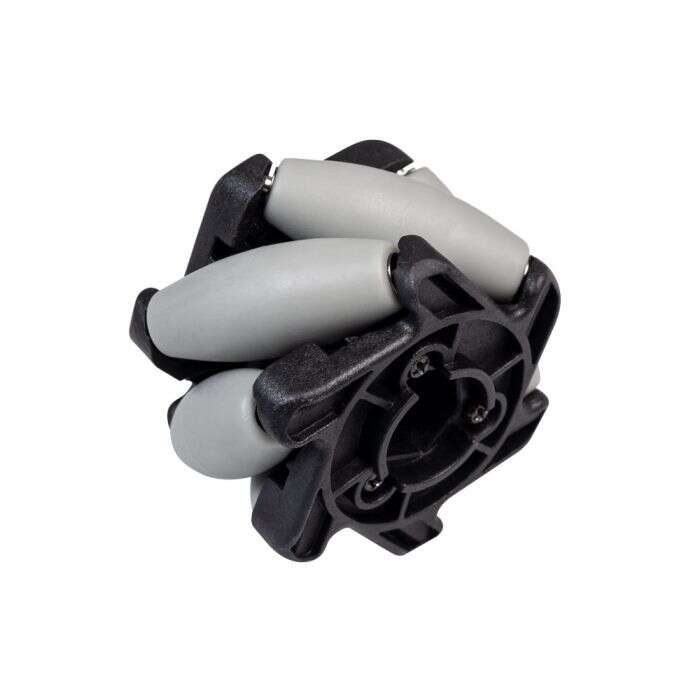
\includegraphics[scale=0.4]{Figures/mecanum1.jpg} 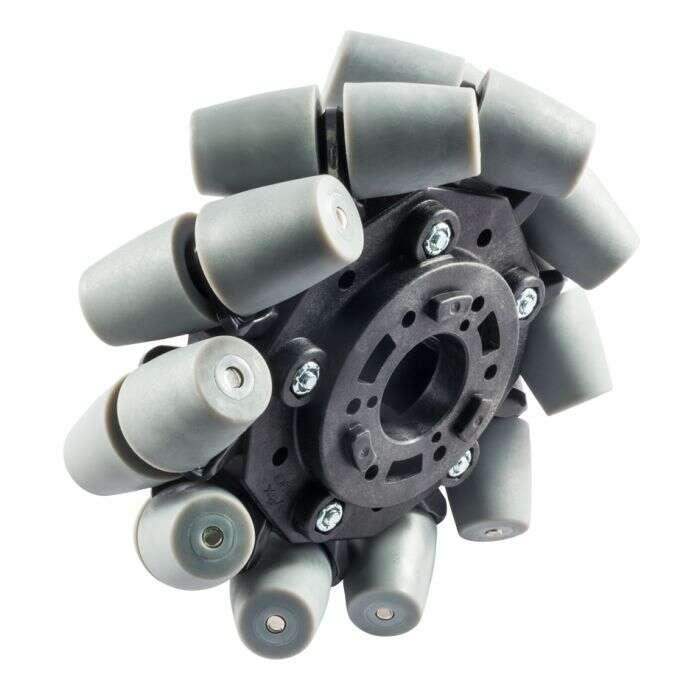
\includegraphics[scale=0.3]{Figures/mecanum2.jpg} 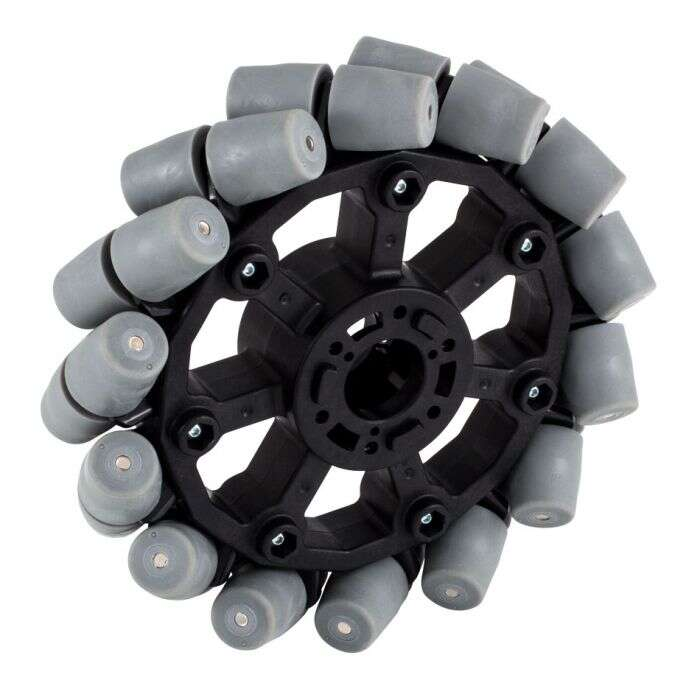
\includegraphics[scale=0.3]{Figures/mecanum3.jpg}\centering
\caption[Different variations of mecanum wheels] {Different variations of mecanum wheels \cite{diegel_improved_nodate}.}
\label{fig:differentvariationsofmecanumwheels}
\end{figure}

In the development of mecanum and other omnidirectional wheels \cite{kim_design_2001}\cite{paromtchik_practical_1994}, undesirable vibrations are frequently present in the motion due to a large number of small rollers on the wheel's periphery.

\subsubsection{Omnidirectional and holonomic motion}

A lot of design work on omnidirectional vehicles has been conducted over the years.
The earliest omnidirectional mobile vehicle to be proposed was based on introducing a methodology for the kinematic modelling of an omnidirectional wheeled mobile robot equipped with four omnidirectional wheels which were based on passive rollers arranged
in an overlapping way \cite{javier_moreno_design_2016}.
These wheels were positioned in pairs on the same axle but with opposite orientations.
Another proposal by Wada and Mori \cite{wada_holonomic_1996} presented a new type of holonomic mobile robot which was equipped with steerable and coordinated driving wheels using conventional tires to provide an omnidirectional capability by actuating the wheels axis and a steering axis independently.
In another paper by Javier Moreno, Eduard Clotet, and others design \cite{javier_moreno_design_2016} validate a three-wheel holonomic motion system for an assistant personal robot.
The paper analyzes the kinematics of the motion system and validates the estimation of the trajectory by comparing the displacement estimated with the internal odometry of the motors and the displacement estimated with a \ac{SLAM} procedure based on \ac{LIDAR} information . 

\subsection{Gap Analysis}

Huge leaps have been made in the development of mobile vehicles or robots with holonomic and omnidirectional motion.
Mecanum wheels have taken center stage, and the use of rollers attached to a conventional wheel has found great applications in small-scale robots and mobile platforms.
However, these wheels cannot be applied to certain applications that involve heavy payloads or rough terrains.
Such applications are moving objects in warehouses or factory floors.
Castors are predominantly used in these areas, but it involves manual control.
This process can be automated by modifying the castors by adding motors for directional control and adding the concept of remote control.
This, however, has not been adopted which necessitates this research.


% \begin{equation}
% \dot{x}=Ax+Bu+B_dw
% \end{equation}
% %
%  Refering a chapter in the main text. For instance Chapter~\ref{sec:review} 
% %
% \begin{eqnarray} \nonumber
% E = 210000\Unit{\mathrm{\frac{N}{mm^2}}}
% \end{eqnarray}
% %

% %
% \begin{eqnarray}
% K_\varphi & = & 3.64\;\mr{\frac{V}{rad}}\quad\mbox{and}\\
% K_x & = & 28.32 \;\mr{\frac{V}{m}}.
% \end{eqnarray}
% %


  \clearpage
    \section{Methodology}
The design considerations will be explored in this section. There will also be a full description of how the smart fan system will be implemented. Figure \ref{fig:architecture} shows the basic architecture of the system. Because it is part of a larger modular system, its integration should be seamless. There are basically two modules:

\begin{itemize}
\item The smart fan
\item The sensor node
\end{itemize}

\begin{figure}[h]
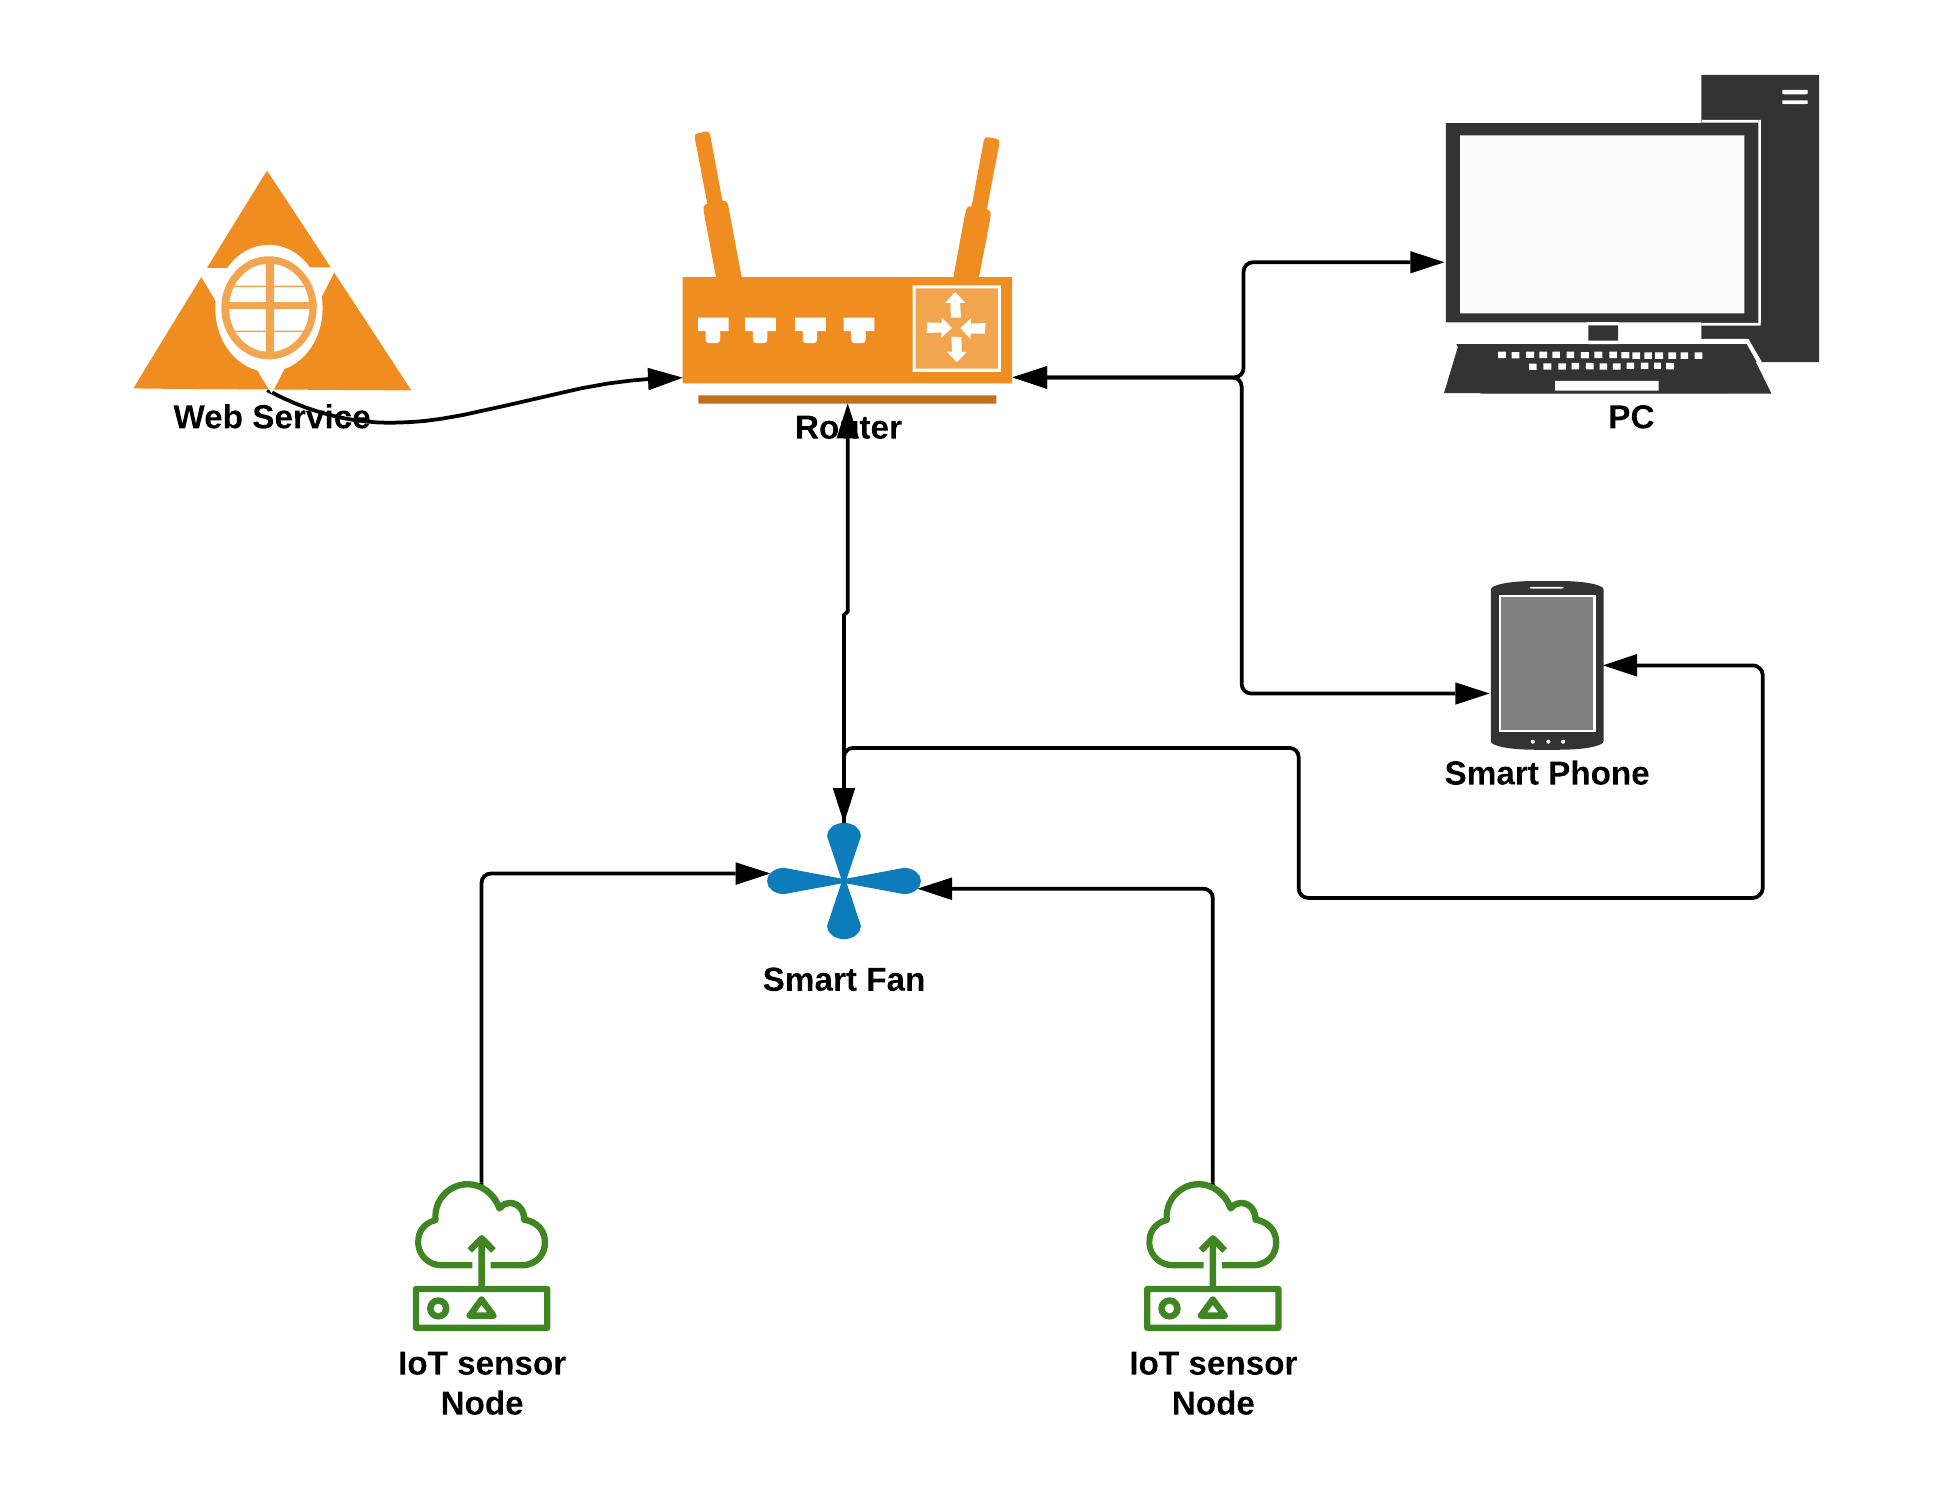
\includegraphics[scale=0.15]{architecture}
\centering
\caption{Design architecture}
\label{fig:architecture}
\end{figure}

The sensor nodes measure the temperature of the room and send it to the smart fan main controller. The sensor nodes are positioned far from the smart fan but in the same room to measure the temperature endpoint after the air has travelled from the smart fan.
\par
The smart fan has the main controller. This controller controls the stepper motor which controls the position of the fan. It also controls the brushless \ac{DC} motor which controls the spinning of the fan. The main controller communicates with sensor nodes via \ac{BLE} then communicates with your device through the \ac{Wi-Fi} router in your home or you can connect to its \ac{Wi-Fi} network.
\par
The following modules break down the design problem:

\subsection{Interface module}

The interface module is responsible for the following:
\begin{itemize}
\item Human-machine interface.
\item Manual overriding of settings and configurations.
\item Creating a visual appeal of the product.
\end{itemize}

The following considerations were made during the design of the interface of the mechanism:
\begin{itemize}
\item Fulfilling the function to control the smart fan remotely.
\item Unlocking the full functionality of the smart fan
\item Ease of use of the interface.
\item Ease of integration with third-party mobile \ac{IoT} applications.
\item Availability on both Android and Web platforms.
\end{itemize}

The interface for this design is intended to be a web and android based application to be installed on the device of the home user. In tandem, it will provide a few buttons to start and stop. This will be crucial to our development as we will provide the user with the ultimate user experience for both advanced and novel users.
The \ac{UX} is a phrase that is strongly related to the \ac{UI}. The distinction between the two is that \ac{UI} is concerned with what a user sees and interacts with, whereas \ac{UX} is concerned with the total experience a user has with a product. It comprises the website, application, hardware packing, and installation, among other things.
\par
The user can receive automatic notifications if they have a web or Android application. In \ac{IoT} applications, the most common scenario is that we want to be notified or alerted if something strange occurs. The user will also be able to keep a proactive eye on the data. The user will undoubtedly be able to control the system remotely as a result of this. This might also be done automatically by the application, based on the instructions provided.

\subsection{Communication module}

The communication module is responsible for the following:

\begin{itemize}
\item Transmitting data from our sensor nodes to the smart fan.
\item Transmitting data from our smart fan to the mobile phone and vice versa.
\item Sending analytics data back to our backend server.
\end{itemize}

The following considerations were made during the design of the interface of the mechanism:

\begin{itemize}
\item Communication must be done over low energy.
\item Communication must be secured with encryption.
\item Communication must be done wirelessly either through \ac{BLE} or \ac{Wi-Fi}.
\end{itemize}

The four most prevalent wireless technologies, \ac{BLE}, \ac{UWB}, ZigBee, and \ac{Wi-Fi}, will be evaluated quantitatively in terms of transmission time, data coding efficiency, protocol complexity, and power consumption in this paper. Network protocol appropriateness is heavily influenced by practical applications but based on existing data, the best technology to be used will be \ac{BLE} Low Energy based on its low consumption power, availability and low overhead.
\par
For communication with the mobile device, \ac{Wi-Fi} will be the appropriate medium. This is based on research that most home users use \ac{Wi-Fi} within their homes and also most of them keep their \ac{Wi-Fi} on connect compared to \ac{BLE} \cite{shimray_use_2019}.
\par
\ac{UART} communication will be used for communication with the \ac{BLE} module. A \ac{UART} provides a bi-directional byte stream so that both ends of a connection can transmit and receive bytes with each other \cite{noauthor_uart_2015}.

\subsection{Software and Processors module}

The software and processing module is responsible for the following:

\begin{itemize}
\item Process information from the interface to actuate it.
\item Control the smart fan.
\item Transmit data to the backend server.
\item Receive data from the sensor nodes.
\item Be able to utilize deep sleep
\item Minimum of 1 \ac{PWM} and \ac{UART} communication pins
\item \ac{Wi-Fi} and \ac{BLE} enabled
\end{itemize}

The following considerations were made during the design of the software and processing module of the mechanism:

\begin{itemize}
\item Computationally less intensive method
\item Secure all communications
\item Low cost of the processors module with \ac{Wi-Fi} and BLE modules
\end{itemize}

Figure \ref{fig:softwarelogic} shows the basic software logic of how the smart fan control module will operate.

\begin{figure}[t]
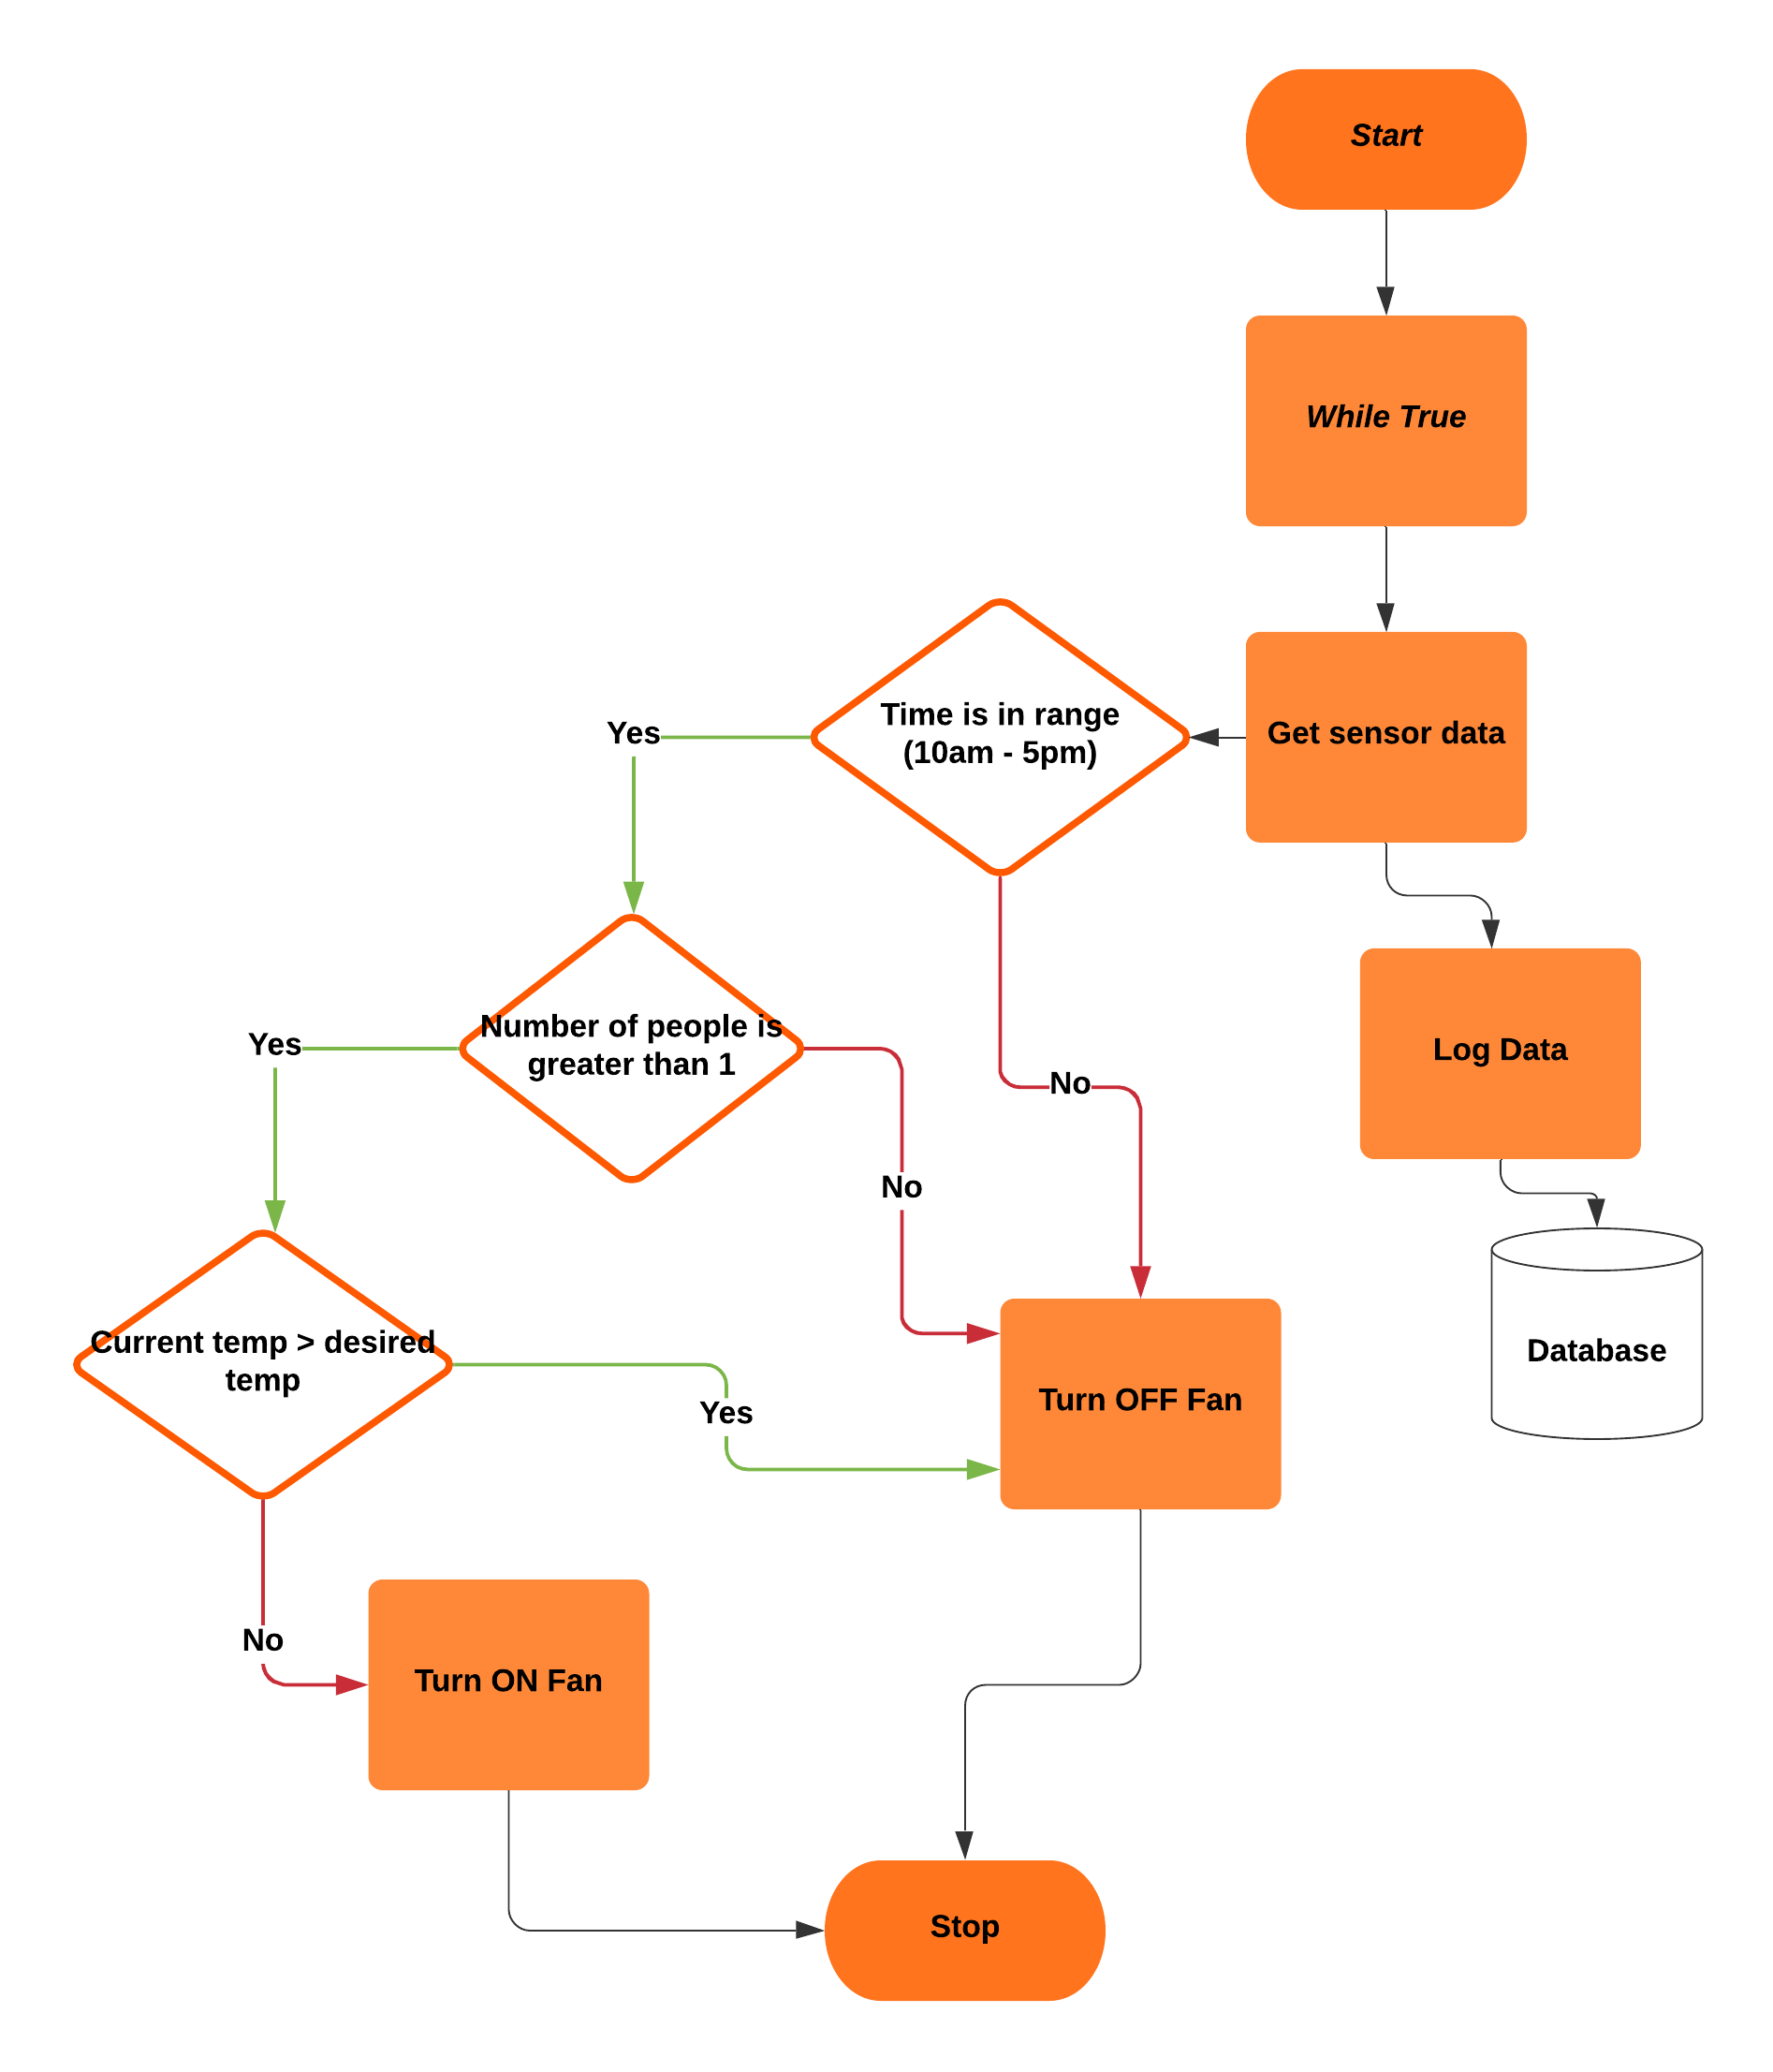
\includegraphics[scale=0.15]{Figures/logic.png}
\centering
\caption{Software Logic}
\label{fig:softwarelogic}
\end{figure}

\subsection{Measurement module}

The interface module is responsible for the following:
\begin{itemize}
\item Measure temperature and humidity.
\item Identify the occupants in the house.
\end{itemize}

The following considerations were made during the design of the measurement module of the mechanism:
\begin{itemize}
\item Fulfilling the function to control the smart fan remotely.
\item Unlocking the full functionality of the smart fan.
\item Ease of use of the interface.
\end{itemize}

\subsection{Actuation module}

The actuation module is responsible for the following:

\begin{itemize}
\item Rotating the Brushless \ac{DC} motor.
\item Rotating the Stepper Motor.
\end{itemize}


\subsection{Assembly module}

The assembly module is responsible for the following:
\begin{itemize}
\item Synergistic integration of the motor and fan blades.
\item Full working of the sensor nodes.
\item Hold the fan up high and maintain its weight.
\end{itemize}

The following considerations were made during the design of the assembly of the mechanism:
\begin{itemize}
\item Use as many modular parts as possible.
\item Using easily available material from the workshops.
\item Must hold the frame so as not to fall.
\end{itemize}

The fan will be assembled by mountain the fan blades on the motor shaft. The fan casing will be added onto the fan blades, while the motor is added into the motor casing. This will be assembled to the stand so as to hold it above. The stand will have an aluminium tube and a base plate to increase stability.
\par
The fan blades will be constructed from a \ac{PVC} tube. The tube will be cut and straightened out after which the blades with equal dimensions will be cut out and rolled to have a curvature. This is to reduce the air resistance as the fan is moving. The blades will be attached to the centre case which will be attached to the motor shaft.
\par
The fan case will be made from small steel wires welded together. It will be moulded into a punched shape and mounted to the motor mount as the fan will be inside the case.
\par
The stand, made from a steel tube, will be joined to the motor mount, hence holding the fan in position. 
\par
For the sensor node, the \ac{PCB} circuitry will be assembled inside the sensor box which will be \ac{3D} printed. A battery will be added to provide power to the sensor node. 

\subsection{Environment module}

The environment module is responsible for the following:

\begin{itemize}
\item Interaction with the environment.
\item Blow maximum air through the inlet diffuser
\end{itemize}

The following considerations were made during the design of the environment module of the mechanism:
\begin{itemize}
\item To minimise noise produced by the fan as it moves.
\item Not to interfere with most of the user’s space
\item Ultimately reduce energy consumption hence helping reduce climate change at large.
\end{itemize}

For the design, the motor should produce the minimum noise possible while rotating. Its aesthetics will be improved by applying paint which will increase the product appeal to the user.
The sensor nodes will also interact with the environment, getting temperature readings from it. The sensor node will be as small as possible and not interfere with the aesthetics of the room.















  \clearpage
    \section{Expected Outcomes}

\begin{enumerate}
\item Fabricated fan blades, fan case, motor mount and stand of the smart fan.
\item Synergistic Integration of a stepper motor and a brushless dc motor to the motor mount and fan blades.
\item An algorithm to control the rotation of the fan blades based on the temperature, position and number of people in a room.
\item An application receipt to \ac{KEBS} for our product.

\end{enumerate}



%  \clearpage
%  \section{Appendices}
  \clearpage
%----  Bibliography  ----------------------------------------
\markright{References}                               % Erzeugt Kopfzeile
\addcontentsline{toc}{section}{References}            % L                     % BIBTeX
\bibliographystyle{Bib/IEEEtran}
\bibliography{Bib/References.bib}

\nocite{Lun02}
                                     % Falls etwas in die Literaturliste soll, was nicht Referenziert wird
                                     
\clearpage
\pagestyle{myheadings}

\markright{APPENDICES}                               % Erzeugt 
\addcontentsline{toc}{section}{Appendices}            % L           

% \section{Appendices}

\section*{Appendix A: Time plan}
% \textbf{Appendix A: Time plan}
%width=0.7\linewidth
\begin{figure}[hb]
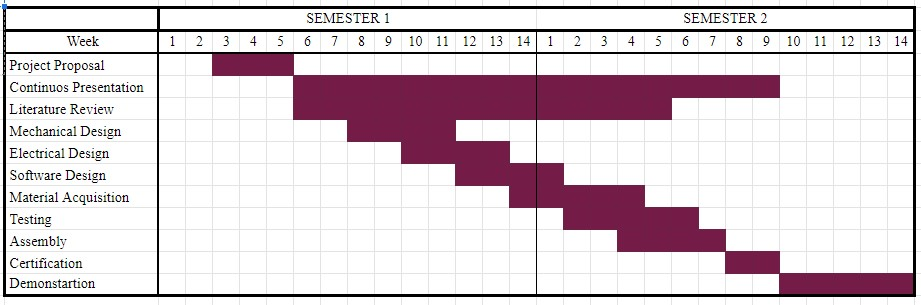
\includegraphics[scale=0.6]{Figures/timeplane.jpg}
\centering
\caption{Timeplan}
\label{fig:timeplan}
\end{figure}

\section*{Appendix B: Budget}

\begin{figure}[hb]
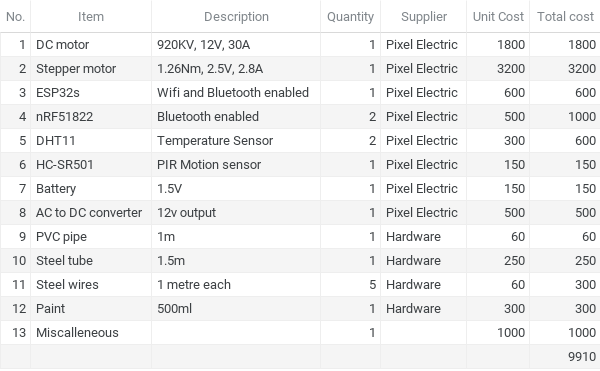
\includegraphics[scale=0.5]{Figures/budget.png}
\centering
\caption{Budget}
\label{fig:budget}
\end{figure}

% \begin{table}[ht]
%   \begin{center}
%     \leavevmode
%      \begin{tabular}{ | p{1cm} | c | p{1cm} | c | c | c | }
%      \hline
% 	No. & Item & Qty & Supplier & Unit Cost & Total cost\\
% 	\hline
% 	1 & DC motor & 1 & Pixel Electric & 1800 & 1800\\ \hline
% 	2 & Stepper motor & 1 & Pixel Electric & 3200 & 3200\\ \hline
% 	3 & ESP32s & 1 & Pixel Electric & 600 & 600\\ \hline
% 	4 & nRF51822 & 2 & Pixel Electric & 500 & 1000\\ \hline
% 	5 & DHT11 & 2 & Pixel Electric & 300 & 600\\ \hline
% 	6 & HC-SR501 & 1 & Pixel Electric & 150 & 150\\ \hline
% 	7 & Battery & 1 & Pixel Electric & 150 & 150\\ \hline
% 	8 & AC to DC converter & 1 & Pixel Electric & 500 & 500\\ \hline
% 	9 & 1m PVC pipe & 1 & Hardware & 60 & 60\\ \hline
% 	10 & 1.5m Steel tube & 1 & Hardware & 250 & 250\\ \hline
% 	11 & 1m Steel wires & 5 & Hardware & 60 & 300\\ \hline
% 	12 & 500ml Paint & 1 & Hardware & 300 & 300\\ \hline
% 	13 & Miscalleneous & 1 &  & 1000 & 1000\\ \hline
% 	14 &  &  &  & TOTAL & 9910\\ \hline
%     \end{tabular}
%     \hangcaption[Estimated budget]{Estimated budget}
%     \label{table:4}
%   \end{center}
% \end{table}

% \appendix
% \chapter{Appendix}
% 
% \section{Appendices}

\section*{Appendix A: Time plan}
% \textbf{Appendix A: Time plan}
%width=0.7\linewidth
\begin{figure}[hb]
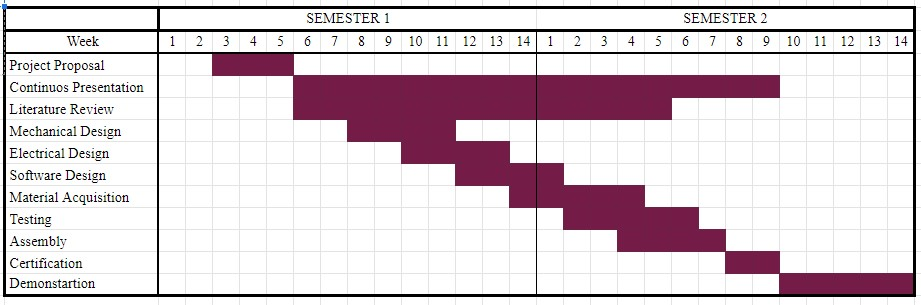
\includegraphics[scale=0.6]{Figures/timeplane.jpg}
\centering
\caption{Timeplan}
\label{fig:timeplan}
\end{figure}

\section*{Appendix B: Budget}

\begin{figure}[hb]
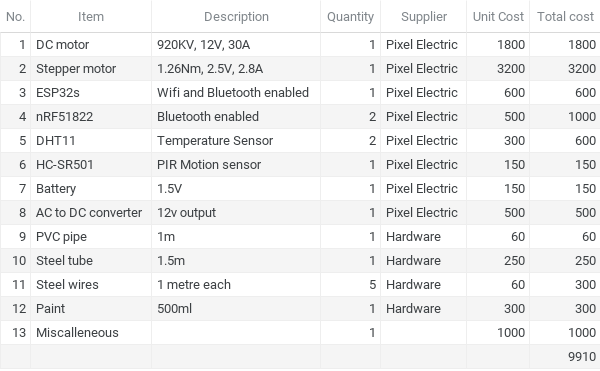
\includegraphics[scale=0.5]{Figures/budget.png}
\centering
\caption{Budget}
\label{fig:budget}
\end{figure}

% \begin{table}[ht]
%   \begin{center}
%     \leavevmode
%      \begin{tabular}{ | p{1cm} | c | p{1cm} | c | c | c | }
%      \hline
% 	No. & Item & Qty & Supplier & Unit Cost & Total cost\\
% 	\hline
% 	1 & DC motor & 1 & Pixel Electric & 1800 & 1800\\ \hline
% 	2 & Stepper motor & 1 & Pixel Electric & 3200 & 3200\\ \hline
% 	3 & ESP32s & 1 & Pixel Electric & 600 & 600\\ \hline
% 	4 & nRF51822 & 2 & Pixel Electric & 500 & 1000\\ \hline
% 	5 & DHT11 & 2 & Pixel Electric & 300 & 600\\ \hline
% 	6 & HC-SR501 & 1 & Pixel Electric & 150 & 150\\ \hline
% 	7 & Battery & 1 & Pixel Electric & 150 & 150\\ \hline
% 	8 & AC to DC converter & 1 & Pixel Electric & 500 & 500\\ \hline
% 	9 & 1m PVC pipe & 1 & Hardware & 60 & 60\\ \hline
% 	10 & 1.5m Steel tube & 1 & Hardware & 250 & 250\\ \hline
% 	11 & 1m Steel wires & 5 & Hardware & 60 & 300\\ \hline
% 	12 & 500ml Paint & 1 & Hardware & 300 & 300\\ \hline
% 	13 & Miscalleneous & 1 &  & 1000 & 1000\\ \hline
% 	14 &  &  &  & TOTAL & 9910\\ \hline
%     \end{tabular}
%     \hangcaption[Estimated budget]{Estimated budget}
%     \label{table:4}
%   \end{center}
% \end{table}


\end{document}
